\subsection{Sliding Window Approach}
blindtext

\subsection{Temporal Models}
blindtext

\begin{table}[H]
    \centering
    \resizebox{\textwidth}{!}{
    \begin{tabular}{lccccccc}
        \hline
        \rowcolor{white} \textbf{Model} & \textbf{original Autocrop} & \textbf{Switch 1} & \textbf{Switch 2} & \textbf{Switch 3} & \textbf{Switch 4} & \textbf{AVG all Switches} & \textbf{AVG Switch 1 \& 3} \\
        \hline
        \rowcolor[gray]{0.9} TEP Net \cite{tepNet2024}    & \checkmark & 22.10 \%          & 18.47 \%          & 63.96 \%          & \textbf{94.76 \%} & 49.82 \%          & 43.03 \%          \\ 
        \rowcolor{white}     single-frame-based           &            & 22.43 \%          &  3.68 \%          & 65.99 \%          & 81.99 \%          & 43.53 \%          & 44.21 \%          \\ 
        \rowcolor[gray]{0.9} single-frame-based           & \checkmark & 22.57 \%          & 18.56 \%          & 63.85 \%          & 82.74 \%          & 46.93 \%          & 43.21 \%          \\ 
        \hline
        \rowcolor[gray]{0.9} CNN\_FC\_LSTM                &            & 23.89 \%          &  6.77 \%          & 70.01 \%          & 84.47 \%          & 46.29 \%          & 46.95 \%          \\ 
        \rowcolor{white}     CNN\_LSTM\_V1                &            & 26.40 \%          &  4.70 \%          & \textbf{83.77 \%} & 69.55 \%          & 46.10 \%          & 55.09 \%          \\ 
        \rowcolor[gray]{0.9} CNN\_LSTM\_V2                &            & 32.11 \%          &  0.64 \%          & 78.86 \%          & 79.15 \%          & 42.79 \%          & 43.30 \%          \\ 
        \rowcolor{white}     CNN\_LSTM\_HEAD              &            & \textbf{40.59 \%} &  3.05 \%          & 78.32 \%          & 78.33 \%          & 47.69 \%          & 55.49 \%          \\ 
        \rowcolor[gray]{0.9} CNN\_FC\_FCOUT\_V1           &            & 25.11 \%          &  2.71 \%          & 61.49 \%          & 81.86 \%          & 50.07 \%          & \textbf{59.46 \%} \\ 
        \rowcolor{white}     CNN\_FC\_FCOUT\_V2           &            & 23.59 \%          &  3.76 \%          & 61.82 \%          & 86.68 \%          & 47.76 \%          & 56.18 \%          \\ 
        \rowcolor[gray]{0.9} CNN\_FLAT\_FC                &            & 30.47 \%          &  0.46 \%          & 81.88 \%          & 78.24 \%          & 43.96 \%          & 42.70 \%          \\ 
        \rowcolor{white}     CNN\_LSTM\_SKIP\_CAT         &            & 22.58 \%          &  2.08 \%          & 70.02 \%          & 82.83 \%          & 44.38 \%          & 46.30 \%          \\ 
        \rowcolor[gray]{0.9} CNN\_LSTM\_SKIP\_MUL\_FRAME  &            & 22.29 \%          &  3.18 \%          & 72.55 \%          & 84.38 \%          & 45.60 \%          & 47.42 \%          \\ 
        \rowcolor{white}     CNN\_LSTM\_SKIP\_MUL\_TIME   &            & 21.49 \%          &  5.52 \%          & 65.90 \%          & 83.96 \%          & 44.22 \%          & 43.69 \%          \\ 
        \hline
        \rowcolor[gray]{0.9} CNN\_FC\_LSTM                & \checkmark & 23.65 \%          & \textbf{23.43 \%} & 70.35 \%          & 88.23 \%          & \textbf{51.41 \%} & 47.00 \%          \\ 
        \rowcolor{white}     CNN\_LSTM\_V1                & \checkmark & 26.22 \%          & 14.82 \%          & 80.69 \%          & 72.51 \%          & 48.56 \%          & 53.46 \%          \\ 
        \rowcolor[gray]{0.9} CNN\_LSTM\_V2                & \checkmark & 28.50 \%          & 13.44 \%          & 76.83 \%          & 75.99 \%          & 45.72 \%          & 39.42 \%          \\ 
        \rowcolor{white}     CNN\_LSTM\_HEAD              & \checkmark & 30.61 \%          &  9.93 \%          & 80.15 \%          & 76.68 \%          & 48.69 \%          & 52.66 \%          \\ 
        \rowcolor[gray]{0.9} CNN\_FC\_FCOUT\_V1           & \checkmark & 23.40 \%          & 20.43 \%          & 55.45 \%          & 83.60 \%          & 49.34 \%          & 55.38 \%          \\ 
        \rowcolor{white}     CNN\_FC\_FCOUT\_V2           & \checkmark & 21.40 \%          & 20.07 \%          & 59.29 \%          & 85.92 \%          & 50.60 \%          & 54.25 \%          \\ 
        \rowcolor[gray]{0.9} CNN\_FLAT\_FC                & \checkmark & 27.80 \%          & 13.35 \%          & 80.70 \%          & 80.54 \%          & 46.67 \%          & 40.35 \%          \\ 
        \rowcolor{white}     CNN\_LSTM\_SKIP\_CAT         & \checkmark & 22.92 \%          &  4.43 \%          & 78.36 \%          & 85.37 \%          & 47.77 \%          & 50.64 \%          \\ 
        \rowcolor[gray]{0.9} CNN\_LSTM\_SKIP\_MUL\_FRAME  & \checkmark & 22.85 \%          &  2.27 \%          & 77.05 \%          & 86.57 \%          & 47.18 \%          & 49.95 \%          \\ 
        \rowcolor{white}     CNN\_LSTM\_SKIP\_MUL\_TIME   & \checkmark & 22.53 \%          & 18.34 \%          & 64.79 \%          & 85.35 \%          & 47.75 \%          & 43.66 \%          \\ 
        \hline
    \end{tabular}
    }
    \caption{Temporal Models Results IoUs}
    \label{tab:temporalModelsResultsIoUs}
\end{table}


\begin{table}[H]
    \centering
    \resizebox{\textwidth}{!}{
    \begin{tabular}{lcccccccccc}
        \hline
        \rowcolor{white} \textbf{Model} & \textbf{Testset} & \textbf{Sequence 1} & \textbf{Sequence 2} & \textbf{Sequence 3} & \textbf{Sequence 4} & \textbf{Switch 1} & \textbf{Switch 2} & \textbf{Switch 3} & \textbf{Switch 4} & \textbf{switch averages} \\
        \hline
        \rowcolor[gray]{0.9} single-frame-based           & 57.03 \%          & 60.66 \%          & 2.06 \%                            & 76.75 \%                            & 88.66 \%                            & 22.43 \%                            & 3.60 \%                            & 65.99 \%                            & 81.99 \%                            & 43.5 \%\\ 
        \hline
        \rowcolor{white}     CNN\_LSTM\_FC                & \multicolumn{10}{c}{canceled at epoch 107: no generalization} \\ 
        \rowcolor[gray]{0.9} CNN\_FC\_LSTM                & 52.88 \%          & 43.60 \%          & \textcolor{blue}{4.22 \%}          & 74.71 \%                            & \textcolor{blue}{88.99 \%}          & \textcolor{blue}{23.89 \%}          & \textcolor{blue}{\textbf{6.61 \%}} & \textcolor{blue}{70.01 \%}          & \textcolor{blue}{84.47} \%          & 46.25 \% \\ 
        \rowcolor{white}     CNN\_LSTM\_V1                & 52.93 \%          & 45.80 \%          & \textcolor{blue}{3.42 \%}          & \textcolor{blue}{85.19 \%}          & 77.29 \%                            & \textcolor{blue}{26.40 \%}          & \textcolor{blue}{4.59 \%}          & \textcolor{blue}{\textbf{83.77 \%}} & 69.55 \%                            & 46.08 \% \\ 
        \rowcolor[gray]{0.9} CNN\_LSTM\_V2                & 50.96 \%          & 41.50 \%          & 0.76 \%                            & \textcolor{blue}{80.08 \%}          & 81.49 \%                            & \textcolor{blue}{32.11 \%}          & 0.62 \%                            & \textcolor{blue}{78.86 \%}          & 79.15 \%                            & 42.78 \% \\ 
        \rowcolor{white}     CNN\_LSTM\_HEAD              & 52.04 \%          & 44.34 \%          & \textcolor{blue}{2.19 \%}          & \textcolor{blue}{80.19 \%}          & 81.44 \%                            & \textcolor{blue}{\textbf{40.59 \%}} & 2.98 \%                            & \textcolor{blue}{78.32 \%}          & 78.33 \%                            & 47.69 \% \\ 
        \rowcolor[gray]{0.9} CNN\_FC\_FCOUT\_V1           & 50.57 \%          & 43.88 \%          & \textcolor{blue}{\textbf{5.49 \%}} & 68.44 \%                            & 84.47 \%                            & \textcolor{blue}{25.11 \%}          & 2.65 \%                            & 61.49 \%                            & 81.86 \%                            & 50.05 \% \\ 
        \rowcolor{white}     CNN\_FC\_FCOUT\_V2           & 53.35 \%          & 50.59 \%          & \textcolor{blue}{4.05 \%}          & 68.22 \%                            & \textcolor{blue}{\textbf{90.52 \%}} & \textcolor{blue}{23.59 \%}          & \textcolor{blue}{3.67 \%}          & 61.82 \%                            & \textcolor{blue}{\textbf{86.68 \%}} & 47.76 \% \\ 
        \rowcolor[gray]{0.9} CNN\_FLAT\_FC                & 50.17 \%          & 42.81 \%          & 0.75 \%                            & \textcolor{blue}{83.01 \%}          & 74.08 \%                            & \textcolor{blue}{30.47 \%}          & 0.45 \%                            & \textcolor{blue}{81.88 \%}          & 78.24 \%                            & 43.94 \% \\ 
        \rowcolor{white}     CNN\_LSTM\_SKIP\_CAT         & 56.17 \%          & 56.27 \%          & 1.17 \%                            & \textcolor{blue}{78.66 \%}          & 88.58 \%                            & \textcolor{blue}{22.58 \%}          & 2.03 \%                            & \textcolor{blue}{70.02 \%}          & \textcolor{blue}{82.83 \%}          & 44.37 \% \\ 
        \rowcolor[gray]{0.9} CNN\_LSTM\_SKIP\_MUL\_FRAME  & \textbf{56.97 \%} & 56.31 \%          & 1.79 \%                            & \textcolor{blue}{\textbf{80.27 \%}} & \textcolor{blue}{89.51 \%}          & 22.29 \%                            & 3.11 \%                            & \textcolor{blue}{72.55 \%}          & \textcolor{blue}{84.38 \%}          & 45.58 \% \\ 
        \rowcolor{white}     CNN\_LSTM\_SKIP\_MUL\_TIME   & 56.41 \%          & \textbf{57.12 \%} & \textcolor{blue}{3.41 \%}          & 75.68 \%  	                         & \textcolor{blue}{89.45 \%}          & \textcolor{blue}{21.49 \%}          & \textcolor{blue}{5.39 \%}          & 65.90 \%                            & \textcolor{blue}{83.96 \%}          & 44.18 \% \\ 
        \hline
        \rowcolor[gray]{0.9} best with MNV3-Small & xy \% & xy \% & xy \% & xy \% & xy \% & xy \% & xy \% & xy \% & xy \% & xy \% \\
        \rowcolor{white}     best with MNV3-Large & xy \% & xy \% & xy \% & xy \% & xy \% & xy \% & xy \% & xy \% & xy \% & xy \% \\
        \hline
    \end{tabular}
    }
    \caption{Temporal Models Results IoUs}
    \label{tab:temporalModelsResultsIoUs_old}
\end{table}

\begin{table}[H]
    \centering
    \resizebox{\textwidth}{!}{
    \begin{tabular}{lcccc}
        \hline
        \rowcolor{white} \textbf{} & \textbf{Switch 1} & \textbf{Switch 2} & \textbf{Switch 3} & \textbf{Switch 4} \\
        \hline
        \rowcolor[gray]{0.9} TEP \cite{tepNet2024} IoU                                                      & 22.10 \%      & 18.47 \%          & 63.96 \%    & 94.76 \% \\
        \rowcolor{white}     improved single-frame-based model IoU                                          & 22.43 \%      &  3.68 \%          & 65.99 \%    & 81.99 \% \\
        \rowcolor[gray]{0.9} improved single-frame-based model with original autocrop \cite{tepNet2024} IoU & 22.57 \%      & 18.56 \%          & 63.85 \%    & 82.74 \% \\
        \rowcolor{white}     best temporal model                                                            & CNN\_LSTM\_HEAD & CNN\_FC\_LSTM (ogA) & CNN\_LSTM\_V1 & CNN\_FC\_LSTM (ogA) \\
        \rowcolor[gray]{0.9} best temporla model IoU                                                        & 40.59 \%      & 23.43 \%          & 83.77 \%    & 88.23 \% \\
        \hline
    \end{tabular}
    }
    \caption{Temporal Models Results Switches}
    \label{tab:temporalModelsResultsSwitches}
\end{table}

\begin{figure}[H]
    \centering
    % Erste Reihe
    \begin{subfigure}[b]{0.49\textwidth}
        \centering
        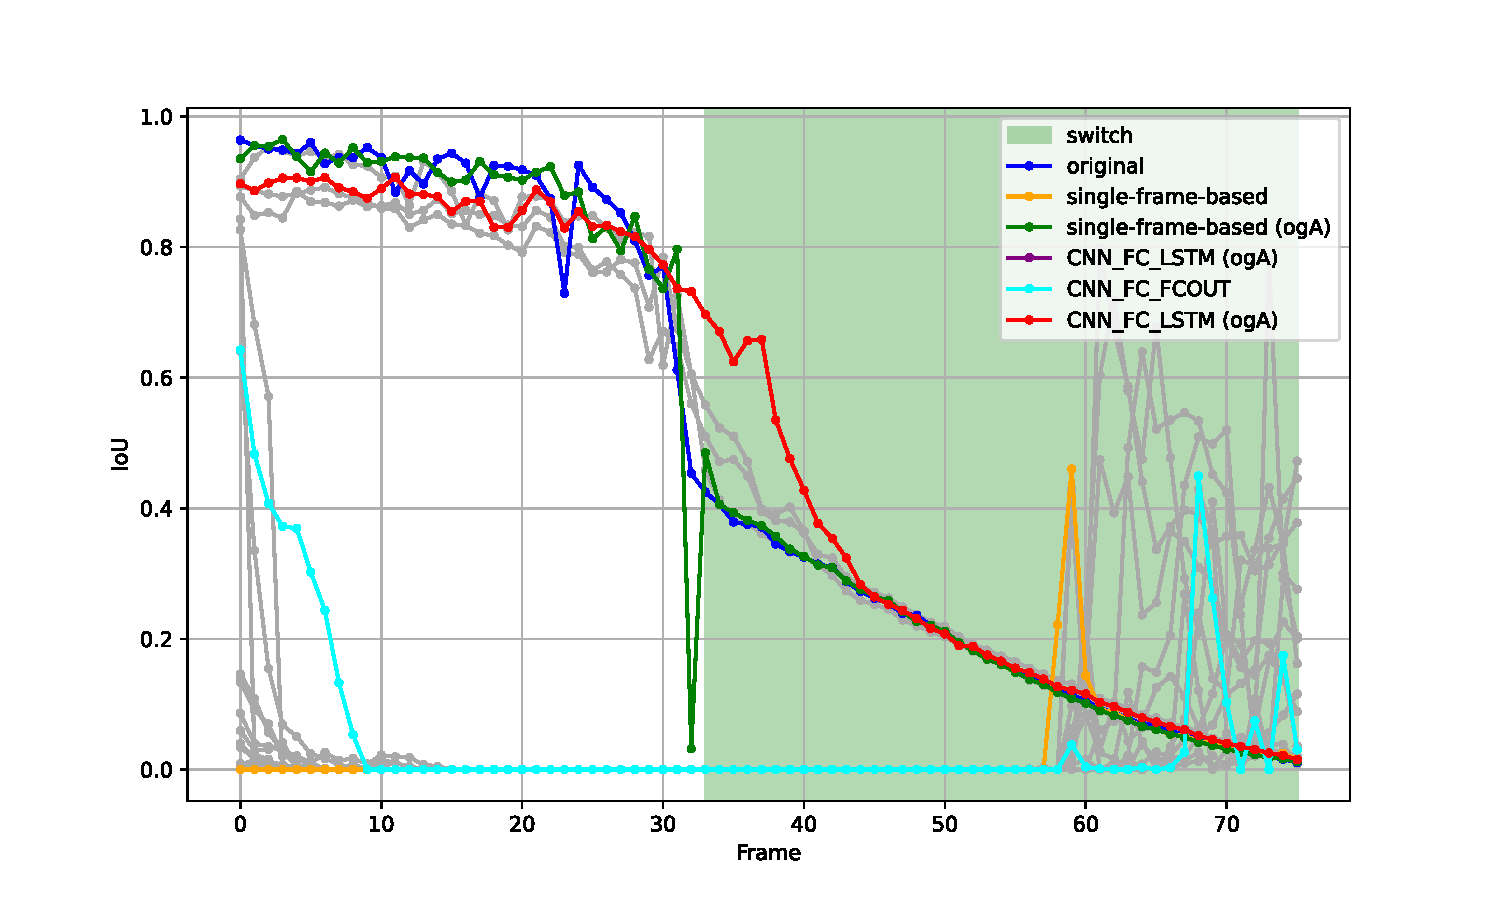
\includegraphics[width=\textwidth]{PICs/experiments/temporalModels/plot_ious_sequence_2.pdf}
        \caption{Beschreibung 1}
        \label{fig:grafik1}
    \end{subfigure}
    %\hfill
    \begin{subfigure}[b]{0.49\textwidth}
        \centering
        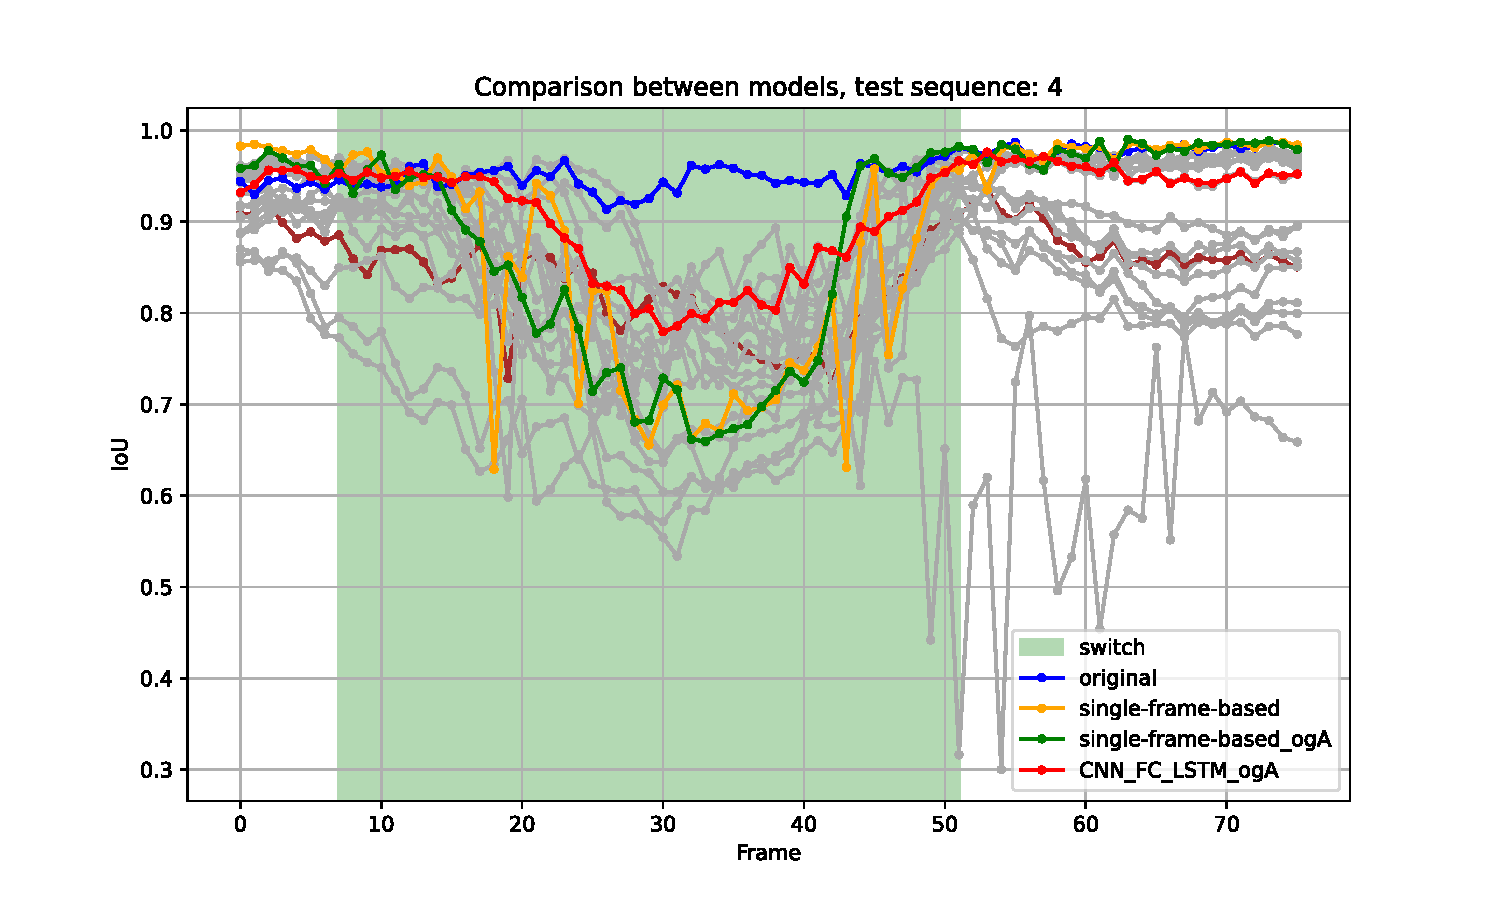
\includegraphics[width=\textwidth]{PICs/experiments/temporalModels/plot_ious_sequence_4.pdf}
        \caption{Beschreibung 2}
        \label{fig:grafik2}
    \end{subfigure}

    \vspace{1em} % Vertikaler Abstand zwischen den Reihen

    % Zweite Reihe
    \begin{subfigure}[b]{1\textwidth}
        \centering
        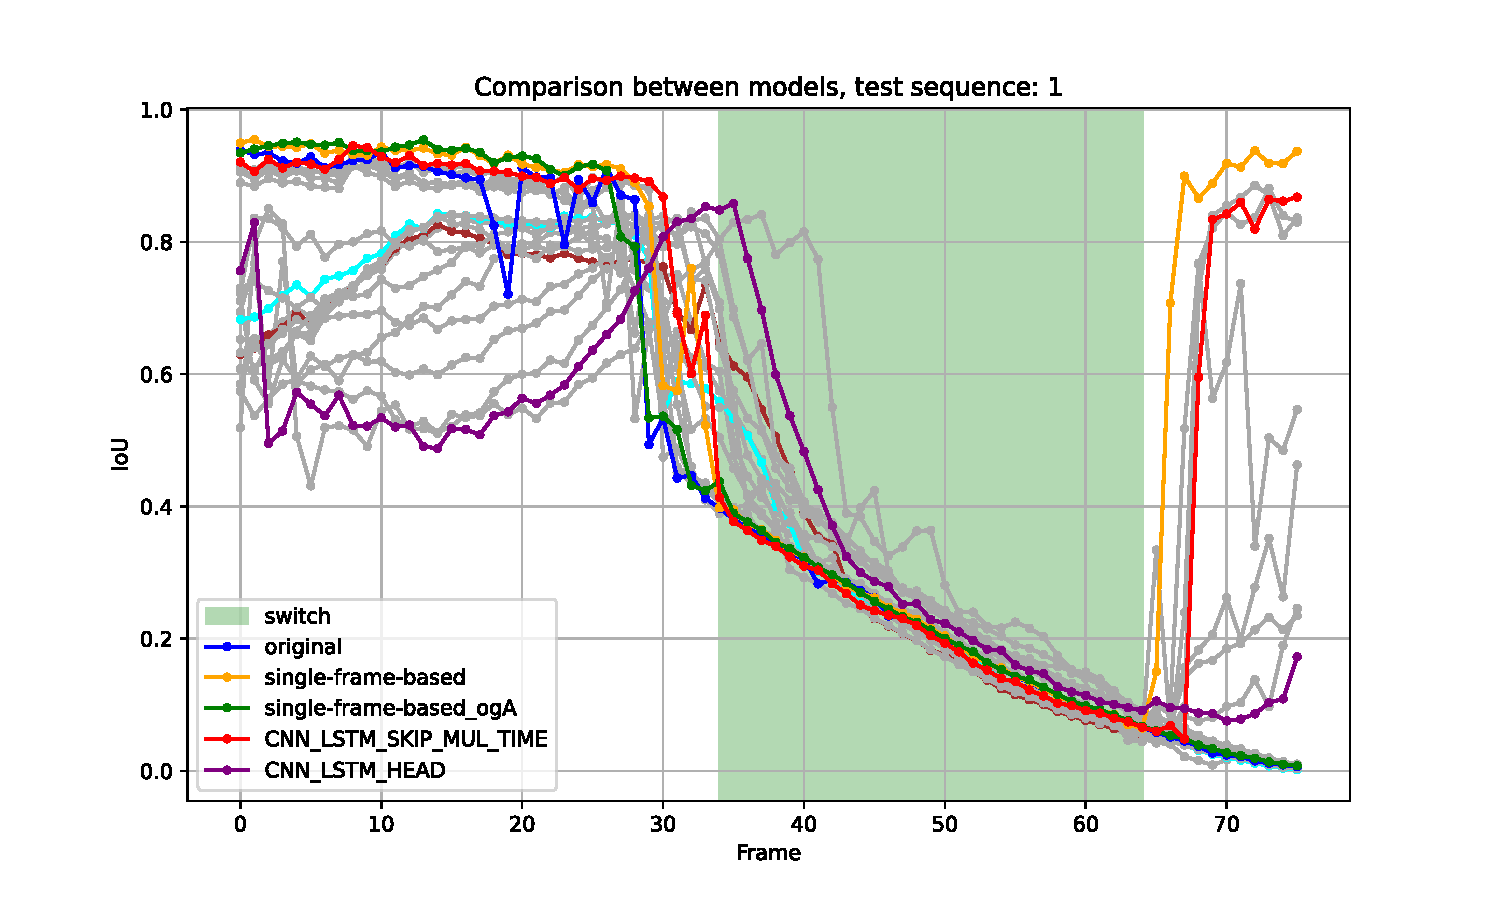
\includegraphics[width=0.8\textwidth]{PICs/experiments/temporalModels/plot_ious_sequence_1.pdf}
        \caption{Beschreibung 3}
        \label{fig:grafik3}
    \end{subfigure}
    %\hfill
    \begin{subfigure}[b]{1\textwidth}
        \centering
        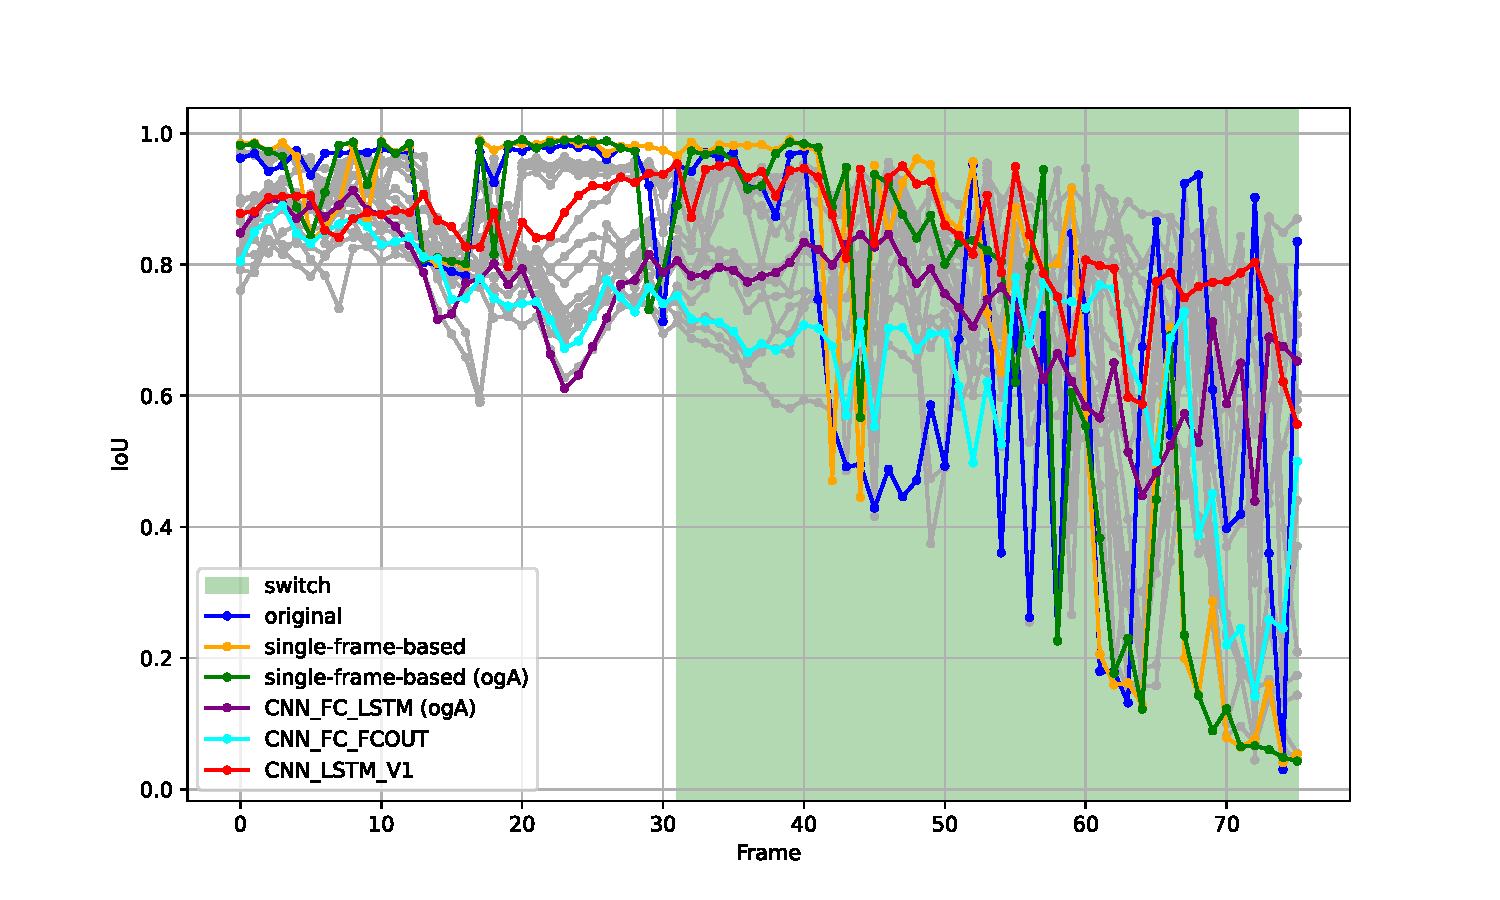
\includegraphics[width=0.8\textwidth]{PICs/experiments/temporalModels/plot_ious_sequence_3.pdf}
        \caption{Beschreibung 4}
        \label{fig:grafik4}
    \end{subfigure}

    \caption{Titel für alle vier Grafiken}
    \label{fig:4grafiken}
\end{figure}


\begin{table}[H]
    \centering
    \resizebox{\textwidth}{!}{
    \begin{tabular}{lcccc}
        \hline
        \rowcolor{white} \textbf{Model} & \textbf{Parameters} & \textbf{Flops} & \textbf{MACs} & \textbf{Latency TRT FP32 / FP16} \\
        \hline
        \rowcolor[gray]{0.9} single-frame-based          & 32.92M & 10.17B & 5.38G & 25.87 / 16.09 ms \\ 
        \hline
        \rowcolor{white}     CNN\_LSTM\_FC               & \multicolumn{4}{c}{canceled at epoch 107: no generalization} \\ 
        \rowcolor[gray]{0.9} CNN\_FC\_LSTM               & 32.87M  & 101.72B & 53.81G & \textbf{223.07} / 129.69 ms \\ 
        \rowcolor{white}     CNN\_LSTM\_V1               & \textbf{11.10M}  & \textbf{101.28B} & \textbf{53.59G} & 246.90 / 156.04 ms \\ 
        \rowcolor[gray]{0.9} CNN\_LSTM\_V2               & 13.62M  & 101.33B & 53.62G & 246.94 / 155.09 ms \\ 
        \rowcolor{white}     CNN\_LSTM\_HEAD             & 13.15M  & 101.32B & 53.61G & 247.11 / 136.35 ms \\ 
        \rowcolor[gray]{0.9} CNN\_FC\_FCOUT\_V1          & 33.08M  & 101.72B & 53.81G & 265.14 / 128.91 ms \\ 
        \rowcolor{white}     CNN\_FC\_FCOUT\_V2          & 35.50M  & 101.72B & 53.81G & 328.86 / 156.09 ms \\ 
        \rowcolor[gray]{0.9} CNN\_FLAT\_FC               & 132.21M & 101.52B & 53.71G & 230.06 / \textbf{127.88} ms \\ 
        \rowcolor{white}     CNN\_LSTM\_SKIP\_CAT        & 35.05M  & 101.36B & 53.63G & 223.87 / 131.76 ms \\ 
        \rowcolor[gray]{0.9} CNN\_LSTM\_SKIP\_MUL\_FRAME & 35.04M  & 101.76B & 53.83G & 227.75 / 130.14 ms \\ 
        \rowcolor{white}     CNN\_LSTM\_SKIP\_MUL\_TIME  & 35.05M  & 101.76B & 53.83G & 265.56 / 130.15 ms \\ 
        \hline
        \rowcolor[gray]{0.9} best with MNV3-Small & xyM & xyB & xyG & xy / xy ms \\
        \rowcolor{white}     best with MNV3-Large & xyM & xyB & xyG & xy / xy ms \\
        \hline
    \end{tabular}
    }
    \caption{Temporal Models Results}
    \label{tab:temporalModelsResults}
\end{table}